\documentclass{csse4400}

% \teachermodetrue

\usepackage{languages}

\title{Storing Stuff}
\author{Brae Webb}

\date{\week{3}}
\begin{document}

\maketitle

\begin{figure}[h]
  \href{https://www.oreilly.com/library/view/designing-data-intensive-applications/9781491903063/ch02.html}{
    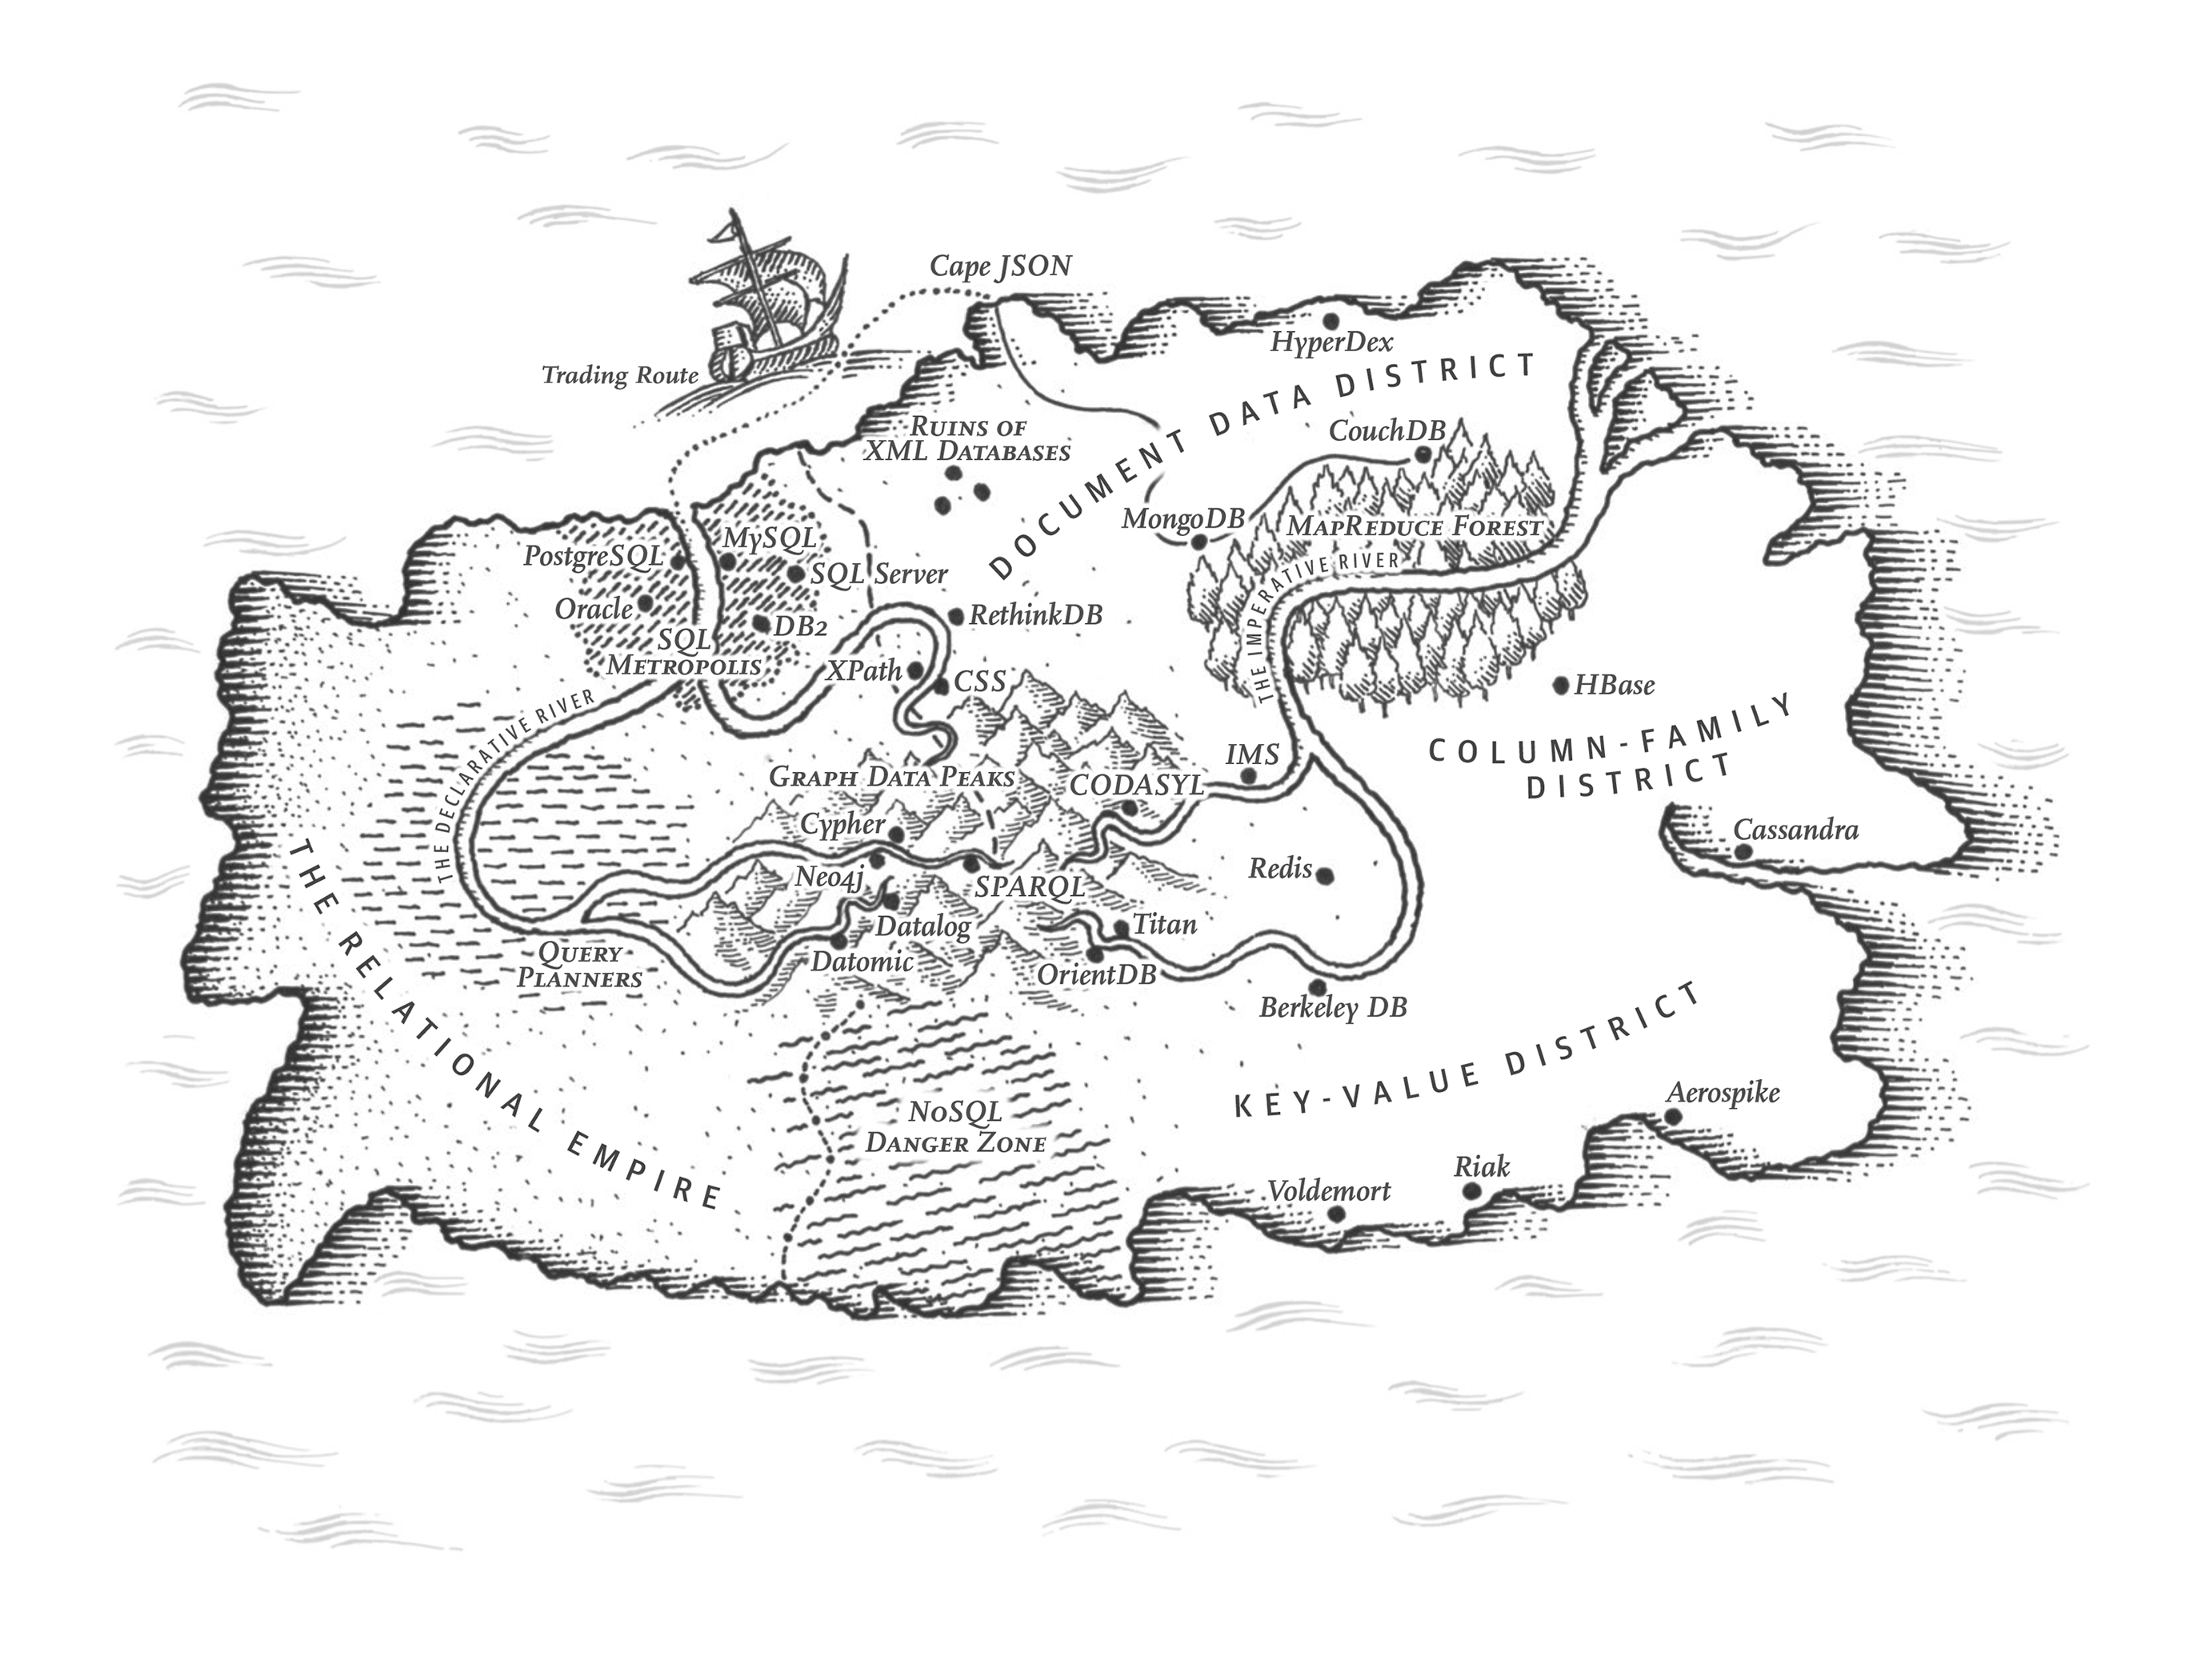
\includegraphics[width=\textwidth]{images/databases}
  }
\caption{A map of data storage techniques from Designing Data-Intensive Applications \cite{data-intensive}.}
\end{figure}

\warning{
  This document is still a work in progress.
}

\section{This Week}
This week our goal is to:
\begin{itemize}
  \item explore the various techniques developers use to store data; and
  \item look at the storage options implementing these techniques on the AWS platform.
  \item run a small application using docker that requires a database.
  \item deploy a small application that requires a database in AWS using Terraform.
\end{itemize}

\section{Introduction}
Unfortunately, to build interesting software we often need to store and use data.
The storage of data introduces a number of challenges to designing, creating, and maintaining our software.
However, not all data storage techniques are created equal;
the choice of data storage model can have a profound impact on our software's complexity and maintainability.
In this practical, we want to take a superficial exploration our island of data storage models.
For a more in-depth treatment of data storage models that is outside the scope of this course,
see the \textit{Designing Data-Intensive Applications} book \cite{data-intensive}.

\section{Relational Storage}
\begin{itemize}
  \item MySQL/MariaDB [ Amazon RDS / Amazon Aurora ].
  \item Postgres [ Amazon RDS / Amazon Aurora ].
\end{itemize}

  \subsection{ORM}
  Just mentioning the relational-object mismatch.

\section{Wide-Column Storage}
  \begin{itemize}
    \item Apache Cassandra [ Amazon Keyspaces for Cassandra ].
    \item Apache HBase.
  \end{itemize}

\section{Key-Value Storage}
\begin{itemize}
  \item Redis [ Amazon ElastiCache for Redis ].
  \item Memcached [ Amazon ElastiCache for Memcached].
  \item Amazon DynamoDB.
  \item Amazon MemoryDB for Redis.
\end{itemize}

\section{Time Series Storage}
\begin{itemize}
  \item Amazon Timestream.
  \item TimescaleDB ( Postgres + Addon ).
  \item Prometheus.
\end{itemize}

\section{Document Storage}
\begin{itemize}
  \item MongoDB.
  \item Apache CouchDB.
  \item Amazon DocumentDB.
\end{itemize}

\section{Graph Storage}
\begin{itemize}
  \item Amazon Neptune.
  \item Neo4J.
  \item Janus Graph.
\end{itemize}

\section{Working with Docker}

So far in the course we have introduced docker as a means to package software to make it easier to work with and deploy.
Today we will be using it to run a small application locally that is a webserver + a database.

\info{
    You will need to have docker and docker-compose installed for this practical.
    Installation will depend on your operating system.

    \begin{itemize}
      \item docker compose: https://docs.docker.com/compose/install/
      \item docker engine: https://docs.docker.com/get-docker/
    \end{itemize}
    
    We also recommend installing the vscode docker plugin or the equlivant tools in IntelliJ IDEs.
}

\notice{
    For terminal examples in this section, lines that begin with a \$ indicate a line which you should 
    type while the other lines are example output that you should expect. Not all of the output is captured 
    in the examples to save on space.  
}

\subsection{Locally}

We will be using a container that is built from the Dockerfile descibed below which can be found here: 
\url{https://github.com/CSSE6400/todo-app/blob/main/backend/Dockerfile}. []

\begin{code}[language=docker]{Dockerfile}
FROM ubuntu:21.10
RUN apt-get update \
        && DEBIAN_FRONTEND=noninteractive apt install -y \
            php \
            php-mysql \
            php-xml \
            php-curl \
            curl \
            git \
            unzip
RUN curl -sS https://getcomposer.org/installer | php -- --install-dir=/usr/local/bin --filename=composer
COPY . /app
WORKDIR /app
RUN composer install
CMD ["php", "artisan", "serve", "--host=0.0.0.0"]
\end{code}

\begin{code}[language=docker-compose]{main.tf}
version: '3.3'
services:
  backend:
    image: ghcr.io/csse6400/todo-app:latest
    ports:
      - '8000:8000'
    environment:
      APP_ENV: 'local'
      APP_KEY: 'base64:8PQEPYGlTm1t3aqWmlAw/ZPwCiIFvdXDBjk3mhsom/A='
      APP_DEBUG: 'true'
      LOG_LEVEL: 'debug'
\end{code}

\begin{code}[language=shell,numbers=none]{}
  $ docker-compose up
  Creating network "p1_default" with the default driver
  Creating p1_backend_1 ... done
  Attaching to p1_backend_1
  backend_1  | Starting Laravel development server: http://0.0.0.0:8000
  backend_1  | [Sun Mar 20 07:56:23 2022] PHP 8.0.8 Development Server (http://0.0.0.0:8000) started
\end{code}

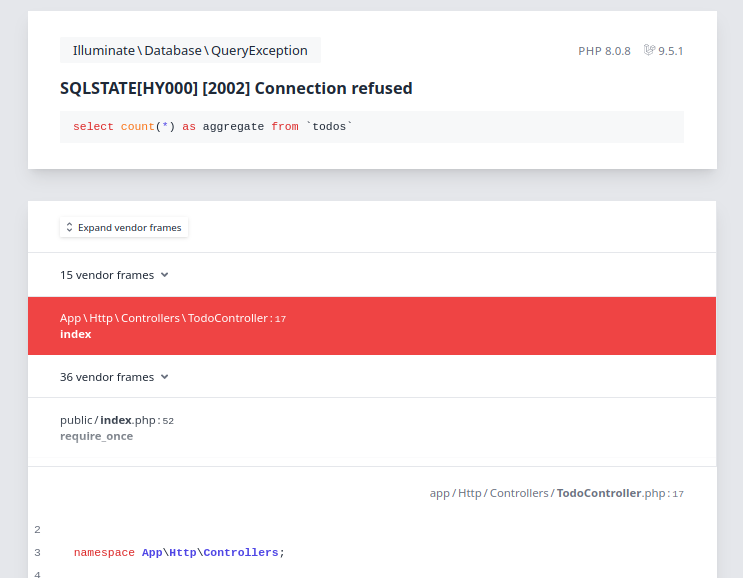
\includegraphics[width=\textwidth]{images/missing-db}

\begin{code}[language=docker-compose]{main.tf}
version: '3.3'
services:
  db:
    image: mysql:8-debian
    environment:
      MYSQL_DATABASE: 'todoapp'
      MYSQL_USER: 'todoapp'
      MYSQL_PASSWORD: 'password'
      MYSQL_ROOT_PASSWORD: 'password'
    ports:
      - '3306:3306'

  backend:
    image: ghcr.io/csse6400/todo-app:latest
    depends_on:
      - db
    ports:
      - '8000:8000'
    environment:
      APP_ENV: 'local'
      APP_KEY: 'base64:8PQEPYGlTm1t3aqWmlAw/ZPwCiIFvdXDBjk3mhsom/A='
      APP_DEBUG: 'true'
      LOG_LEVEL: 'debug'
      DB_CONNECTION: 'mysql'
      DB_HOST: 'db'
      DB_PORT: '3306'
      DB_DATABASE: 'todoapp'
      DB_USERNAME: 'todoapp'
      DB_PASSWORD: 'password'
\end{code}

\begin{code}[language=shell,numbers=none]{}
  $ docker-compose up
  Starting p2_db_1 ... done
  Starting p2_backend_1 ... done
  Attaching to p2_db_1, p2_backend_1
  db_1       | 2022-03-20 08:11:55+00:00 [Note] [Entrypoint]: Entrypoint ....
  db_1       | 2022-03-20 08:11:55+00:00 [Note] [Entrypoint]: Switching t....
  db_1       | 2022-03-20 08:11:55+00:00 [Note] [Entrypoint]: Entrypoint ....
  db_1       | 2022-03-20T08:11:55.438996Z 0 [System] [MY-010116] [Server....
  db_1       | 2022-03-20T08:11:55.445261Z 1 [System] [MY-013576] [InnoDB....
  backend_1  | Starting Laravel development server: http://0.0.0.0:8000
  db_1       | 2022-03-20T08:11:55.535803Z 1 [System] [MY-013577] [InnoDB....
  db_1       | 2022-03-20T08:11:55.673757Z 0 [Warning] [MY-010068] [Serve....
  db_1       | 2022-03-20T08:11:55.673784Z 0 [System] [MY-013602] [Server....
  db_1       | 2022-03-20T08:11:55.674810Z 0 [Warning] [MY-011810] [Serve....
  db_1       | 2022-03-20T08:11:55.684729Z 0 [System] [MY-010931] [Server....
  db_1       | 2022-03-20T08:11:55.684756Z 0 [System] [MY-011323] [Server....
  backend_1  | [Sun Mar 20 08:11:55 2022] PHP 8.0.8 Development Serv....
\end{code}

\todo{ Going to 127.0.0.1:8000/api/v1/todo will show an error page }

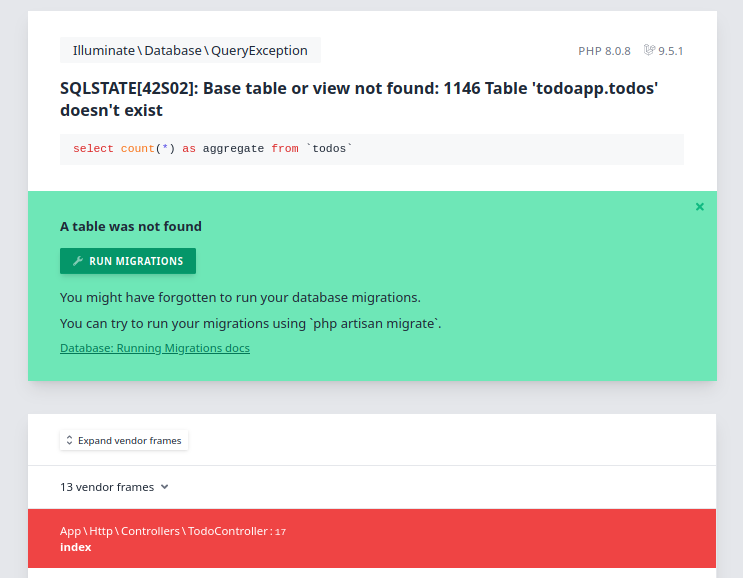
\includegraphics[width=\textwidth]{images/missing-tables}

\begin{code}[language=shell,numbers=none]{}
$ docker-compose exec backend php artisan migrate:fresh --seed
Dropped all tables successfully.
Migration table created successfully.
Migrating: 2022_03_19_041557_create_todos_table
Migrated:  2022_03_19_041557_create_todos_table (7.55ms)
Seeding: Database\Seeders\TodoSeeder
Seeded:  Database\Seeders\TodoSeeder (6.56ms)
Database seeding completed successfully.
\end{code}

\subsubsection{Exercise: Migrations at startup}

So far when we run this application we have to perform the database migrations manually. To help us get up and running
we are going to make a small modification to pre run the migrations when are web app starts. First we need to have a look
at how the container is set to launch by default. In the Dockerfile attached at the start of the prac we see that we have
defined the command to run on the last line with the CMD directive.

\begin{code}[language=docker]{Dockerfile}
  FROM ubuntu:21.10
  ... 
  ... 
  ...
  CMD ["php", "artisan", "serve", "--host=0.0.0.0"]
\end{code}

\info{
  When working with docker it can get confusing around the networking aspects. In this application I have specified
  that the server must listen on all network interfaces ( 0.0.0.0 ). Without this flag the default is 127.0.0.1 which
  even though its the localhost the forwarded traffic through the docker container would never reach it.
}

This command launches the laravel development server and listens on all interfaces on the host. We are going to override
this in our docker-compose file so that we run the migrations then start the server. Add the following line to the 
docker-compose.yml that you have been developing during the prac.

\begin{code}[language=docker-compose]{}
  command: sh -c "sleep 30 && php artisan migrate:refresh --seed && php artisan serve --host=0.0.0.0"
\end{code}

This new command does the following:

\begin{itemize}
  \item Waits for the database to be ready in a simple way.
  \item Runs the migrations and seeds the database, as we have seen earlier.
  \item Starts the development server as the container originally did.
\end{itemize}

Example: redacted version of goal docker-compose.yml attached below.

\begin{code}[language=docker-compose]{docker-compose.yml}
  version: '3.3'
  services:
    db:
      ...
  
    backend:
      ...
      environment:
        ...
      command: sh -c "sleep 10 && php artisan migrate:refresh --seed && php artisan serve --host=0.0.0.0"
\end{code}

Now when we launch the docker-compose we can see that our migrations were run in the output.

\begin{code}[language=shell,numbers=none]{}
  $ docker-compose up
  ...
  ...
  backend_1  | Rolling back: 2022_03_19_041557_create_todos_table
  backend_1  | Rolled back:  2022_03_19_041557_create_todos_table (8.28ms)
  backend_1  | Migrating: 2022_03_19_041557_create_todos_table
  backend_1  | Migrated:  2022_03_19_041557_create_todos_table (11.55ms)
  backend_1  | Seeding: Database\Seeders\TodoSeeder
  backend_1  | Seeded:  Database\Seeders\TodoSeeder (44.77ms)
  backend_1  | Database seeding completed successfully.
  backend_1  | Starting Laravel development server: http://0.0.0.0:8000
  backend_1  | [Sun Mar 20 12:08:41 2022] PHP 8.0.8 Development Server (http://0.0.0.0:8000) started
\end{code}

We can also bake this into the container by extending the original, it is fairly common to see projects
in the wild that run a init script when the container launches. An exercise left for the reader is to 
build upon the provided docker container but create an init script.

\subsection{AWS}

\warning{
  This section is still being developed.
}

\bibliographystyle{ieeetr}
\bibliography{books}

\end{document}